\chapter{Системийн шаардлага}

Энэхүү бүлэгт annotation болон reflection механизмд суурилсан dependency injection framework-ийн шаардлагыг тодорхойлно. Уг framework нь component классуудыг автоматаар илрүүлэх, container-д бүртгэх, dependency-г шийдэх, bean-ийн lifecycle-ийг удирдах суурь түвшний боломжуудыг хэрэгжүүлэхэд чиглэнэ. Иймээс энэ бүлэгт framework-ийн функциональ болон функциональ бус шаардлагууд, хэрэглээний үндсэн үйл явц, боломжит классууд, CRC карт, классын диаграммыг тус тус тодорхойлно.

\section{Framework-ийн шаардлагын тодорхойлолт}

\subsection{Ерөнхий шаардлага}

Хөгжүүлэх framework нь Java хэл дээр хэрэгжих бөгөөд annotation болон reflection механизмд тулгуурлан dependency injection-ийн суурь үйл ажиллагааг хэрэгжүүлнэ. Framework-ийн үндсэн зорилго нь хэрэглэгчийн тодорхойлсон классуудыг package түвшинд илрүүлэх, annotation-уудыг унших, bean болгон бүртгэх, объект үүсгэх, dependency-г автоматаар оноох, улмаар хэрэглэгчид бэлэн объектыг container-оос авах боломж олгоход оршино.

Энэ зорилгын хүрээнд framework нь дараах үндсэн боломжуудыг дэмжсэн байна:
\begin{itemize}
    \item custom annotation-уудыг runtime үед унших,
    \item package scanning хийх,
    \item bean бүртгэх,
    \item singleton болон prototype төлөвийг удирдах,
    \item dependency injection гүйцэтгэх,
    \item bean-ийг нэр болон төрлөөр хайж авах,
    \item алдааг тодорхой exception-оор боловсруулах.
\end{itemize}

\subsection{Функциональ шаардлага}
Функциональ шаардлага нь framework-ийн заавал хийж гүйцэтгэх үндсэн үйлдлүүдийг тодорхойлно. Энэхүү framework нь сургалтын болон судалгааны зориулалттай суурь DI container тул Spring Framework-ийн бүх боломжийг бус, харин dependency injection-ийн гол цөм механизмуудыг хэрэгжүүлэхэд чиглэнэ.
\begin{table}[H]
\centering
\small
\setlength{\tabcolsep}{4pt}
\caption{Framework-ийн функциональ шаардлага}
\label{tab:framework-functional-requirements}
\renewcommand{\arraystretch}{1.3}
\begin{tabularx}{\textwidth}{|L{0.14\textwidth}|L{0.24\textwidth}|Y|}
\hline
\textbf{ID} & \textbf{Шаардлагын нэр} & \textbf{Тодорхойлолт} \\ \hline
ФШ-10 & Package scanning & Заасан package болон түүний дэд package-уудаас класс илрүүлэх боломжтой байна. \\ \hline
ФШ-11 & Annotation detection & \texttt{@Component}, \texttt{@Autowired}, \texttt{@Qualifier}, \texttt{@Scope} annotation-уудыг runtime үед илрүүлдэг байна. \\ \hline
ФШ-12 & Bean registration & \texttt{@Component} тэмдэглэгээтэй классуудыг container-д bean хэлбэрээр бүртгэдэг байна. \\ \hline
ФШ-13 & Object instantiation & Reflection API ашиглан bean-ийн объектыг автоматаар үүсгэдэг байна. \\ \hline
ФШ-14 & Dependency injection & Constructor болон field түвшний dependency injection дэмждэг байна. \\ \hline
ФШ-15 & Bean retrieval & Bean-ийг нэрээр болон төрлөөр \texttt{getBean()} аргаар авах боломжтой байна. \\ \hline
ФШ-16 & Scope management & Singleton болон prototype scope-ийг дэмждэг байна. \\ \hline
ФШ-17 & Exception handling & Bean үүсгэх, dependency шийдэх үед гарсан алдааг тодорхой exception-оор боловсруулдаг байна. \\ \hline
\end{tabularx}
\end{table}
\section{Функциональ бус шаардлага}

Функциональ бус шаардлага нь framework-ийн чанар, гүйцэтгэл, ашиглахад хялбар байдал, тестлэгдэх чадвар зэрэг шинжүүдийг тодорхойлно. Энэхүү framework нь enterprise түвшний иж бүрэн платформ биш боловч судалгааны ажилд ашиглагдах тул тодорхой чанарын шалгууртай байх ёстой.

\begin{table}[H]
\centering
\small
\setlength{\tabcolsep}{4pt}
\caption{Framework-ийн функциональ бус шаардлагууд}
\label{tab:nonfunctional-requirements}
\renewcommand{\arraystretch}{1.2}
\begin{tabularx}{\textwidth}{|L{1.5cm}|L{2.5cm}|L{2.7cm}|X|}
\hline
\textbf{ID} & \textbf{Ангилал} & \textbf{Шаардлага} & \textbf{Хэмжүүр / Тодорхойлолт} \\ \hline
ФБШ-10 & Гүйцэтгэл & Startup хурд & 10 хүртэл bean-тэй үед container-ийн эхлэлт 100ms-аас бага байна. \\ \hline
ФБШ-11 & Гүйцэтгэл & Bean авах хурд & \texttt{getBean()} дуудлага 1ms-аас бага хугацаанд хариулахуйц байна. \\ \hline
ФБШ-12 & Найдвартай байдал & Circular dependency илрүүлэлт & Тойрог хамаарал илэрсэн тохиолдолд startup үед тодорхой алдаа өгч зогсоно. \\ \hline
ФБШ-13 & Санах ойн удирдлага & Singleton cache & Singleton bean-ийг давтан үүсгэхгүй, cache бүтэц ашиглан хадгална. \\ \hline
ФБШ-14 & Ашиглахад хялбар байдал & API энгийн байдал & \texttt{ApplicationContext} үүсгэхэд зөвхөн package нэр өгөхөд хангалттай байна. \\ \hline
ФБШ-15 & Суурилуулалт & Гуравдагч талын хамааралгүй байдал & Framework нь зөвхөн Java SE орчинд, нэмэлт library-гүй ажиллана. \\ \hline
ФБШ-16 & Тестлэгдэх чадвар & Unit тест & Үндсэн функциональ шаардлага бүр JUnit 5 тестээр баталгаажсан байна. \\ \hline
ФБШ-17 & Тайлбарлагдах чадвар & Лог гаргалт & Startup үед бүртгэгдсэн болон inject хийгдсэн bean-үүдийн мэдээллийг харуулдаг байна. \\ \hline
\end{tabularx}
\end{table}
\normalsize

Эдгээр шаардлагууд нь framework-ийг зөвхөн ажилладаг байхаас гадна ойлгомжтой, туршигдахуйц, өргөтгөх боломжтой байдлаар хэрэгжүүлэхэд чиглэнэ.


\section{Нэмэлт сайжруулалт шаардлагатай уялдах нь}

Нэмэлт хэрэгжүүлэлтийн A1 ажил нь framework-д шинэ давхарга эсвэл шинэ annotation нэмэх шат биш, харин энэ бүлэгт тодорхойлсон шаардлагуудын биелэлтийг \textit{чанарын баталгаажуулалтын} түвшинд батлах шат юм. Өөрөөр хэлбэл A1-ийн хүрээнд одоо байгаа \texttt{ApplicationContext}, \texttt{ClassPathScanner}, \texttt{DependencyInjector}, \texttt{BeanRegistry} болон exception давхаргын зан авирыг салбарласан урсгал бүрээр нь тестэлж, fail-fast алдааны мэдэгдлийг ойлгомжтой болгож, туршилтын бүтцийг давхаргат зохиомжтой уялдуулсан.

Энэ ажлыг шаардлагын түвшинд авч үзвэл дараах уялдаа хамгийн чухал байна. Нэгдүгээрт, \textbf{ФШ-17} буюу алдааг тодорхой exception-оор боловсруулах шаардлага A1 ажлын үед илүү тодорхой хэрэгжиж, bean олдохгүй, олон candidate тохирох, bean үүсгэх үед reflection алдаа гарах, тойрог хамаарал үүсэх зэрэг нөхцөл бүрд ялгаатай мэдэгдэл өгөх байдлаар баталгаажсан. Хоёрдугаарт, \textbf{ФБШ-12} болон \textbf{ФБШ-16}-ын хүрээнд тойрог хамаарал, edge case, нэгж болон интеграцийн тестийн хамрах хүрээ тусгайлан өргөжсөн. Гуравдугаарт, \textbf{ФБШ-17}-ын хувьд startup болон injection үеийн төлөвийг ойлгоход ашиглагдах мэдэгдлүүд илүү тайлбарлагдсан болсноор framework-ийг оношлох чадвар сайжирсан.

\begin{table}[H]
\centering
\small
\setlength{\tabcolsep}{4pt}
\caption{A1 ажлын шаардлагатай уялдсан байдал}
\label{tab:a1-requirement-alignment}
\renewcommand{\arraystretch}{1.3}
\begin{tabularx}{\textwidth}{|L{0.24\textwidth}|L{0.18\textwidth}|Y|}
\hline
\textbf{A1 ажлын чиглэл} & \textbf{Уялдах шаардлага} & \textbf{Тайлбар} \\ \hline
Branch бүрийг тестлэх & ФБШ-12, ФБШ-16 & \texttt{ClassPathScanner}, \texttt{ApplicationContext}, \texttt{DependencyInjector} зэрэг цөм классуудын салбарласан урсгал бүрийг нэгж болон интеграцийн тестээр баталгаажуулна. \\ \hline
Exception мэдэгдлийг баяжуулах & ФШ-17, ФБШ-17 & \texttt{NoSuchBeanException}, \texttt{BeanCreationException}, \texttt{CircularDependencyException} нь bean-ийн нэр, төрөл, боломжит шалтгаан зэрэг оношлох мэдээллийг агуулна. \\ \hline
Тестийн бүтцийг цэгцлэх & ФБШ-16 & Туршилтыг \texttt{unit} болон \texttt{integration} түвшинд ангилснаар давхарга тус бүрийн хариуцлагыг тусгаарлан шалгах боломж бүрдэнэ. \\ \hline
Fail-fast зан авирыг баталгаажуулах & ФШ-14, ФШ-17, ФБШ-12 & Dependency олдохгүй, ambiguity үүсэх, default constructor байхгүй, circular dependency илрэх үед framework startup эсвэл lookup үе шатанд шууд алдаа өгч зогсоно. \\ \hline
\end{tabularx}
\end{table}

Иймээс A1 ажил нь энэ бүлгийн шаардлагыг өөрчлөх бус, харин шаардлагын биелэлтийг хэмжиж, дараагийн A2--A4 ажлуудад найдвартай суурь болгох зорилготой чанарын сайжруулалтын үе шат гэж үзэж болно.


\section{A3 dependency tree ажлын шаардлагатай уялдах нь}

Нэмэлт хэрэгжүүлэлтийн A3 ажил нь framework-ийн одоо байгаа dependency injection механизмыг зөвхөн ``ажиллуулах'' бус, харин түүний дотоод dependency бүтэц, bean хоорондын холбоос, циклийн эрсдэлийг тайлбарлахуйц түвшинд шинжлэх боломжтой болгосон өргөтгөл юм. Өөрөөр хэлбэл A3 ажлын гол зорилго нь bean-үүдийг runtime үед graph бүтэц болгон илэрхийлэх, dependency-г мод хэлбэрээр харуулах, циклийг DFS алгоритмаар илрүүлэх, мөн үүссэн dependency tree-г console, JSON, HTML гэсэн хэд хэдэн ойлгомжтой representation-аар хөгжүүлэгчид хүргэхэд оршино.

Энэ ажлыг шаардлагын түвшинд авч үзвэл өмнө тодорхойлсон package scanning, annotation detection, bean registration, dependency injection, fail-fast алдаа боловсруулалт, тестлэгдэх чадвар, тайлбарлагдах чадвар зэрэг шаардлагууд бүгд A3 ажлын суурь болсон. Ялангуяа dependency tree нь \texttt{BeanRegistry}-д бүртгэгдсэн bean-үүдийн харилцааг нэгтгэн харуулах тул package scanning болон annotation detection-ийн үр дүн бодит графын бүтэц болж хувирч байна. Мөн циклийн DFS илрүүлэлт нь \textbf{ФБШ-12} шаардлагыг илүү бүтэцтэй түвшинд баталгаажуулж, HTML visualization нь \textbf{ФБШ-17} шаардлагын хүрээнд framework-ийн дотоод төлөвийг хүний ойлгох хэлбэрээр харуулах шинэ боломж нэмж өглөө.

\begin{table}[H]
\centering
\small
\setlength{\tabcolsep}{4pt}
\caption{A3 ажлын шаардлагатай уялдсан байдал}
\label{tab:a3-requirement-alignment}
\renewcommand{\arraystretch}{1.3}
\begin{tabularx}{\textwidth}{|L{0.18\textwidth}|L{0.20\textwidth}|Y|}
\hline
\textbf{Уялдах шаардлага} & \textbf{A3 ажлын чиглэл} & \textbf{Тайлбар} \\ \hline
ФШ-10, ФШ-12 & Dependency tree source өгөгдөл & Scanner-аар илэрч, registry-д бүртгэгдсэн bean бүр dependency tree-ийн node болох суурь өгөгдөл болж байна. \\ \hline
ФШ-11, ФШ-14 & Dependency холбоос тогтоох & \texttt{@Autowired} field-үүдийг reflection ашиглан уншиж, bean хооронд dependency edge байгуулж байна. \\ \hline
ФШ-15 & Оношлогооны дэмжлэг & Bean lookup зөв ажиллаж буй үр дүнг tree бүтэц, JSON болон HTML representation-аар баталгаажуулж харагдуулах боломж бүрдэв. \\ \hline
ФБШ-12 & DFS cycle detection & Visited set ба recursion stack ашигласан DFS алгоритм dependency cycle-ийг тайлбарлагдсан хэлбэрээр илрүүлнэ. \\ \hline
ФБШ-16 & Туршилтын баталгаа & DependencyTreeIntegrationTest, EnableIoCIntegrationTest, AutoDetectPackageIntegrationTest зэрэг шинэ тестүүд A3 ажлын урсгалыг баталж байна. \\ \hline
ФБШ-17 & Тайлбарлагдах чадвар & Console tree, JSON export, HTML dashboard нь framework-ийн dependency бүтцийг хөгжүүлэгчид илүү ойлгомжтой болгож байна. \\ \hline
ФБШ-15 & Гуравдагч талын сангүй хэрэгжилт & Dependency tree болон visualization нь зөвхөн JDK болон өөрийн exporter-оор хэрэгжсэн тул анхны технологийн шаардлагыг зөрчөөгүй. \\ \hline
\end{tabularx}
\end{table}

Хүснэгт~\ref{tab:a3-requirement-alignment}-оос харахад A3 ажил нь шинэ боломж нэмсэн ч анхны шаардлагын хүрээнээс ангид биш, харин тэдгээрийн бодит биелэлтийг ажиглах, шинжлэх, тайлбарлах шинэ түвшинд өргөтгөсөн байна. Иймээс A3 ажлыг системийн шинэ функциональ өргөтгөлөөс гадна framework-ийн тайлбарлагдах чадвар, оношлогооны чанарыг өсгөсөн архитектур--шаардлагын уялдаатай сайжруулалт гэж үзэж болно.

Энэхүү ажлын үр дүнд дараах өргөтгөсөн шаардлагуудыг тайланд тусгах шаардлагатай болсон.
\begin{itemize}
    \item \textbf{ФШ-18: Dependency tree generation} -- Container-д бүртгэгдсэн bean-үүдээс dependency tree үүсгэдэг байна.
    \item \textbf{ФШ-19: Dependency visualization export} -- Dependency tree-г console, JSON болон HTML хэлбэрээр гаргах боломжтой байна.
    \item \textbf{ФБШ-18: Observability} -- Framework-ийн dependency бүтэц, root node, dependency холбоос, ашиглагдах байдал зэргийг ойлгомжтой хэлбэрээр тайлбарлах боломжтой байна.
    \item \textbf{ФБШ-19: Visualization without third-party library} -- Dependency tree visualization нь гуравдагч талын UI сан ашиглахгүйгээр зөвхөн Java стандарт сан болон өөрийн exporter-оор хэрэгжсэн байна.
\end{itemize}


\section{Custom annotation-уудын шаардлага}


\subsection{Meta-annotation ашиглах шаардлага}

Custom annotation тодорхойлоход дараах meta-annotation-ууд чухал үүрэгтэй.
\begin{itemize}
    \item \texttt{@Target} -- annotation ямар төрлийн программын элемент дээр хэрэглэгдэхийг заана;
    \item \texttt{@Retention} -- annotation ямар хугацаанд хадгалагдахыг тодорхойлно;
\end{itemize}

Энэхүү framework-ийн хувьд хамгийн чухал нь \texttt{@Target} болон
\texttt{@Retention} юм. Ялангуяа
\codeword{@Retention(RetentionPolicy.RUNTIME)} нь annotation-ийг
программ ажиллах үед Reflection API ашиглан унших боломжийг
бүрдүүлдэг. Хэрэв annotation нь runtime үед хадгалагдахгүй бол
container тухайн классыг bean мөн эсэх, эсвэл ямар dependency inject
хийх шаардлагатайг илрүүлэх боломжгүй болно. Иймээс framework-д
ашиглагдах бүх үндсэн annotation-ууд заавал \texttt{RUNTIME}
retention-тэй байна.


\begin{table}[H]
\centering
\caption{Framework-д хэрэгжүүлэх custom annotation-уудын шаардлага}
\label{tab:custom-annotations}
\renewcommand{\arraystretch}{1.3}
\begin{tabular}{|p{3cm}|p{2.4cm}|p{2.4cm}|p{6.5cm}|}
\hline
\textbf{Annotation} & \textbf{Target} & \textbf{Retention} & \textbf{Зорилго} \\ \hline
\texttt{@Component} & TYPE & RUNTIME & Тухайн классыг container-т bean болгон бүртгэхийг заана. Нэрийг \texttt{value()} атрибутаар өгч болно. \\ \hline
\texttt{@Autowired} & FIELD, CONSTRUCTOR & RUNTIME & Dependency-г автоматаар inject хийхийг тэмдэглэнэ. Bean олдохгүй үед алдаа боловсруулах боломжтой. \\ \hline
\texttt{@Qualifier} & FIELD, PARAMETER & RUNTIME & Ижил төрлийн олон bean байвал яг аль bean-ийг inject хийхийг нэрээр заана. \\ \hline
\texttt{@Scope} & TYPE & RUNTIME & Bean-ийн амьдралын мөчлөгийг тодорхойлно. Энэ ажлын хүрээнд \texttt{singleton} болон \texttt{prototype} төрлийг дэмжинэ. \\ \hline
\end{tabular}
\end{table}



\subsection{Retention policy болон runtime reflection-ийн шаардлага}

\textbf{Дэвшүүлсэн асуулт:} Annotation-д суурилсан framework хэрэгжүүлэх үед яагаад заавал \texttt{RUNTIME} түвшинд хадгалагдаж, reflection ашиглан унших боломжтой байх шаардлагатай байдаг вэ?

\textbf{Хариулт:} \texttt{@Retention} нь annotation ямар хугацаанд хадгалагдахыг тодорхойлдог бөгөөд энэ нь тухайн annotation-ийг программын аль үе шатанд ашиглахыг шийддэг. Өөрөөр хэлбэл annotation зөвхөн эх кодын түвшинд хэрэгтэй юу, компайл хийгдсэн класс файлд хадгалагдах уу, эсвэл программ ажиллаж байх үед runtime орчинд уншигдах шаардлагатай юу гэдгийг ялгаж өгдөг.


Ийм ангилал хийсэн гол шалтгаан нь бүх annotation ижил зориулалттай биш байдагтай холбоотой. Зарим annotation зөвхөн компиляторт зориулсан байдаг бол зарим нь хөгжүүлэлтийн хэрэгсэл, баримтжуулалт, эсвэл runtime үед ажилладаг framework-д зориулсан байдаг. Тиймээс annotation-ийг ашиглах түвшнээс нь хамааруулан ялгаж өгсөн нь Java хэлний уян хатан, зорилгод нийцсэн шийдэл юм.

Энэхүү судалгааны ажлын хувьд \texttt{RUNTIME} policy хамгийн чухал
байр суурь эзэлж байна. Учир нь annotation-д суурилсан DI framework нь
программ ажиллаж эхэлсний дараа л классуудыг илрүүлэх, тэдгээрийн
annotation-ийг шалгах, объект үүсгэх, хамаарлыг холбох зэрэг үйлдлүүдийг
гүйцэтгэдэг. Энэ бүх процесс compile үе шатанд биш, runtime үед
явагддаг. Иймээс framework annotation-уудыг reflection-оор уншихын тулд
заавал \codeword{RetentionPolicy.RUNTIME} тохиргоотой байх шаардлагатай.

Runtime үед reflection ашиглах шаардлагыг дараах үндсэн гурван талаас тайлбарлаж болно.

\subsubsection{Динамик илрүүлэлт}

Framework нь ерөнхий зориулалттай байх ёстой. Өөрөөр хэлбэл framework-ийг ашиглах хөгжүүлэгч ямар классууд үүсгэх, ямар dependency нэмэх, системээ хэрхэн өргөжүүлэхийг framework урьдчилан мэдэх боломжгүй. Иймээс framework нь хэрэглэгчийн шинээр тодорхойлсон классуудыг программ ажиллах мөчид динамикаар илрүүлдэг байх шаардлагатай.

Программ эхлэх үед framework нь classpath-ийг нэгжиж, тодорхой
annotation бүхий классуудыг олж илрүүлнэ. Энэ нь reflection-ийн
хамгийн чухал давуу тал болох динамик чанарыг илэрхийлдэг.
Жишээлбэл, хөгжүүлэгч \codeword{@MyComponent} annotation бүхий шинэ
класс нэмсэн тохиолдолд framework үүнийг compile үе шатанд бус,
runtime үед л бодитоор илрүүлж чадна.

\begin{lstlisting}[language=Java, caption={Reflection ашиглан классыг динамикаар ачаалах жишээ}, label={lst:dynamic-loading}]
Class<?> clazz = Class.forName("com.myapp.UserService");
Object obj = clazz.getDeclaredConstructor().newInstance();
\end{lstlisting}

Энэ нь framework-д уян хатан байдал олгож, хөгжүүлэгчийн тодорхойлсон шинэ бүрэлдэхүүнүүдийг урьдчилан хатуу кодлолгүйгээр ажиллуулах боломж бүрдүүлдэг.

\subsubsection{Fail-fast буюу эрт баталгаажуулалт}

Runtime үед reflection ашиглахын өөр нэг чухал шалтгаан нь framework системийн тохиргоо, хамаарал, объектын бүтэц зэрэгт алдаа байгаа эсэхийг эрт илрүүлэх боломжтой байдагт оршино. Программ compile хийгдэж \texttt{.class} файл үүссэний дараа JVM дээр ажиллах үед framework annotation-уудыг уншиж, dependency-үүдийг шалгаж, шаардлагатай объектуудыг үүсгэнэ.

Энэ үе шатанд хэрэв шаардлагатай dependency олдохгүй, хоёрдмол сонголт үүссэн, эсвэл буруу тохиргоо хийсэн бол framework шууд алдаа өгч зогсох боломжтой. Үүнийг \textit{fail-fast} зарчим гэж үздэг. Энэ нь программыг хожуу шатанд гацах, тодорхойгүй алдаа гаргах эрсдэлийг бууруулж, тохиргооны алдааг эхэнд нь илрүүлэх ач холбогдолтой.

Өөрөөр хэлбэл compile үе шат нь зөвхөн синтакс болон төрөл шалгах үндсэн баталгаажуулалтыг хийдэг бол runtime үе шатанд framework нь архитектурын түвшний баталгаажуулалт хийж байна гэж ойлгож болно. Тиймээс reflection-ийг runtime үед ашиглах нь зөвхөн объект үүсгэх хэрэгсэл биш, мөн dependency graph-ийн зөв байдлыг шалгах механизм болдог.

\subsubsection{Уламжлалт объект үүсгэлтээс ялгарах нь}

Java хэл дээр объектыг ерөнхийдөө хоёр аргаар үүсгэж болно.

\begin{enumerate}
    \item \textbf{Static object creation} -- Хөгжүүлэгч классын нэрийг урьдчилан мэдэж, \texttt{new} түлхүүр үгээр шууд объект үүсгэнэ.
    \item \textbf{Dynamic object creation} -- Классын нэрийг текст хэлбэрээр эсвэл runtime мэдээлэлд үндэслэн авч, reflection ашиглан объект үүсгэнэ.
\end{enumerate}

Жишээлбэл:

\begin{lstlisting}[language=Java, caption={Static ба dynamic object creation-ийн ялгаа}, label={lst:static-vs-dynamic}]
UserService service1 = new UserService(); // static

Class<?> clazz = Class.forName("com.myapp.UserService");
Object service2 = clazz.getDeclaredConstructor().newInstance(); // dynamic
\end{lstlisting}


\newpage

\subsection{ApplicationContext-ийн шаардлага}

ApplicationContext нь framework-ийн төв бүрэлдэхүүн хэсэг бөгөөд IoC container-ийн үүргийг гүйцэтгэнэ. Энэ бүрэлдэхүүн хэсэг нь annotation-уудыг унших, bean-үүдийн мета мэдээллийг хадгалах, объект үүсгэх, dependency inject хийх, мөн хэрэглэгчид bean буцаах бүх үндсэн логикийг удирдана. Иймээс framework-ийн хамгийн чухал шаардлагууд ApplicationContext-т төвлөрнө. 

\subsubsection{ApplicationContext-ийн гүйцэтгэх үндсэн үүрэг}

ApplicationContext нь дараах үндсэн үйлдлүүдийг дэмжсэн байх шаардлагатай.
\begin{enumerate}
    \item \textbf{Эхлүүлэлт} -- хэрэглэгч \texttt{ApplicationContext(String packageName)} хэлбэрээр package нэр дамжуулахад тухайн package болон дэд package-ууд дахь классуудыг автоматаар илрүүлэх;
    \item \textbf{Bean бүртгэл} -- \texttt{@Component} annotation-той классуудыг bean гэж тодорхойлон, тэдгээрийн мета мэдээллийг \texttt{BeanDefinition} хэлбэрээр бүртгэх;
    \item \textbf{Object үүсгэлт} -- singleton scope-той bean-үүдийг нэг удаа үүсгэж cache-д хадгалах;
    \item \textbf{Dependency injection} -- \texttt{@Autowired} annotation-той талбар бүрийн хамаарлыг container-с хайж, Reflection ашиглан inject хийх;
    \item \textbf{Bean retrieval API} -- \texttt{getBean(Class<T>)} болон \texttt{getBean(String)} хэлбэрээр bean буцаах;
    \item \textbf{Алдаа боловсруулалт} -- bean олдохгүй байх, олон тохирох bean илрэх, circular dependency үүсэх зэрэг тохиолдолд тодорхой exception шидэх.
\end{enumerate}

\subsubsection{Bean бүртгэл ба мета мэдээлэл}

Container нь runtime үед илрүүлсэн bean бүрийн тухай дараах мэдээллийг хадгалах шаардлагатай.
\begin{itemize}
    \item bean-ийн нэр,
    \item тухайн bean-д харгалзах класс,
    \item scope-ийн төрөл,
    \item annotation metadata,
    \item singleton тохиолдолд үүссэн instance.
\end{itemize}

Эдгээрийг нэг дор хадгалах үүднээс \texttt{BeanDefinition} хэмээх тусгай бүтэц ашиглах нь оновчтой. \texttt{BeanDefinition} нь bean-ийн бодит объект биш, харин тухайн bean-ийг хэрхэн үүсгэх, ямар шинжтэй болохыг илэрхийлэх мета мэдээллийн объект байна. Ингэснээр container дотоод логикоороо уян хатан ажиллах боломжтой болно.

\subsubsection{Dependency injection-ийн шаардлага}

Dependency injection-ийн хувьд container нь эхлээд шаардлагатай bean-ийг type-аар хайж олох, шаардлагатай тохиолдолд \texttt{@Qualifier} утгаар илүү нарийвчлан сонгох, дараа нь Reflection API ашиглан талбарт утга оноох логиктой байна. Хэрэв bean огт олдохгүй бол \texttt{NoSuchBeanException}, ижил төрлийн олон bean тохирвол тусгай алдаа, харин A $\rightarrow$ B $\rightarrow$ A хэлбэрийн тойрог хамаарал үүсвэл \texttt{CircularDependencyException} шидэх шаардлагатай.

Энэ нь fail-fast зарчмыг хэрэгжүүлж буй хэлбэр юм. Өөрөөр хэлбэл framework нь runtime эхлэлийн үеэр dependency-үүдийн алдааг аль болох эрт илрүүлж, тодорхой мэдэгдэл өгөх ёстой. Энэ шаардлага нь сургалтын болон туршилтын зорилготой framework-ийн хувьд онцгой ач холбогдолтой. 

\subsubsection{Scope удирдлагын шаардлага}

Container нь дор хаяж дараах хоёр төрлийн scope-ийг дэмжинэ.
\begin{itemize}
    \item \textbf{Singleton scope} -- нэг bean нэг л удаа үүсэж, дараагийн бүх хүсэлтэд ижил instance буцаагдана;
    \item \textbf{Prototype scope} -- bean хүсэх бүрд шинэ instance үүсгэнэ.
\end{itemize}

Singleton scope нь container-ийн cache механизмыг шаарддаг бөгөөд энэ нь bean авах хурдыг нэмэгдүүлнэ. Prototype scope нь төлөвтэй объектуудыг тус тусад нь үүсгэх боломж олгодог. Энэхүү хоёр scope нь DI framework-ийн үндсэн lifecycle удирдлагыг харуулахад хангалттай гэж үзэв. 

\subsubsection{ApplicationContext сонгосон үндэслэл}

Spring-ийн архитектурт \texttt{BeanFactory} болон \texttt{ApplicationContext} гэсэн хоёр гол түвшин байдаг. \texttt{BeanFactory} нь хамгийн суурь container бол \texttt{ApplicationContext} нь үүнийг өргөтгөсөн, илүү өндөр түвшний боломжуудтай хувилбар юм. \texttt{ApplicationContext} гэсэн нэршлийг ашиглах нь оновчтой гэж үзэв. Учир нь уг нэршил нь IoC container, bean lifecycle, dependency resolution гэсэн ойлголтуудыг нэгдмэл байдлаар илэрхийлж чадна. Мөн сургалтын түвшинд Spring Framework-тэй харьцуулан тайлбарлахад илүү ойлгомжтой. 
\subsection{Технологийн шаардлага}

Framework-ийн хэрэгжилт нь аль болох гуравдагч талын сангаас хамааралгүй, зөвхөн Java SE стандарт сангууд дээр тулгуурласан байх шаардлагатай. Энэ нь framework-ийн дотоод механизмыг илүү тодорхой харуулах бөгөөд Reflection, class loading, annotation inspection зэрэг гол ойлголтуудыг гаднын abstraction-гүйгээр судлах боломж олгоно. Үүнтэй холбоотойгоор дараах технологийн орчныг сонгов.

\begin{table}[H]
\centering
\caption{Framework хэрэгжүүлэх технологийн шаардлага}
\label{tab:technology-requirements}
\renewcommand{\arraystretch}{1.3}
\begin{tabular}{|p{3.3cm}|p{3.2cm}|p{6.3cm}|}
\hline
\textbf{Ангилал} & \textbf{Хэрэгсэл / Технологи} & \textbf{Тайлбар} \\ \hline
Программчлалын хэл & Java SE 17 (LTS) & Annotation, Reflection, class loading зэрэг механизмыг стандарт түвшинд дэмжинэ. \\ \hline
Build tool & Apache Maven 3.9.x & Төслийн бүтэц, compile, dependency болон test-ийг удирдахад ашиглана. \\ \hline
IDE & IntelliJ IDEA Community Edition & Reflection-д суурилсан кодын debug болон runtime төлөв ажиглахад тохиромжтой. \\ \hline
Тестийн орчин & JUnit 5 & Framework-ийн үндсэн үйлдлүүдэд unit тест бичиж баталгаажуулахад ашиглана. \\ \hline
JVM & OpenJDK 17 / Temurin 17 & Java 17 орчныг тогтвортой ажиллуулах виртуал машин. \\ \hline
Нэмэлт сан & Байхгүй & Зөвхөн JDK стандарт сан ашиглана. \\ \hline
\end{tabular}
\end{table}

\subsubsection{Java 17 сонгосон үндэслэл}

Java 17 нь урт хугацааны дэмжлэгтэй (LTS) хувилбар бөгөөд орчин үеийн Java хөгжүүлэлтэд тогтвортой суурь орчин гэж үзэгддэг. Annotation, Reflection, generics, module system зэрэг энэхүү судалгааны ажилд шаардлагатай боломжуудыг бүрэн дэмждэг. Мөн Java 17 ашигласнаар framework-ийн хэрэгжилт орчин үеийн JVM орчинд туршигдаж, цаашид өргөтгөхөд илүү найдвартай суурь бүрдэнэ.

\subsubsection{IntelliJ IDEA сонгосон үндэслэл}

Энэхүү framework-ийн хэрэгжилт нь runtime үед Reflection API ашиглан класс илрүүлэх, annotation шалгах, private field-д хандах, объект үүсгэх зэрэг олон шаттай далд логик агуулна. Иймээс хөгжүүлэлтийн орчин нь зөвхөн код бичих хэрэгсэл байхаас гадна санах ой дахь объектын төлөвийг ажиглах, алхамчилсан debug хийх, stack trace болон exception-ийн урсгалыг шинжлэх боломжтой байх ёстой.

Энэ шаардлагын үүднээс IntelliJ IDEA нь илүү оновчтой орчин гэж үзэв. Учир нь уг IDE нь Java төслүүдийн бүтцийг сайн таньдаг, Maven-тэй нягт уялддаг, мөн Reflection-д суурилсан логикийг алхам алхмаар мөрдөж шалгахад тохиромжтой. Харин Eclipse болон VS Code нь тодорхой нөхцөлд ашиглаж болох боловч runtime inspection болон deep debugging-ийн хувьд IntelliJ IDEA илүү давуу гэж үзэж байна.

\subsubsection{Гуравдагч талын сан ашиглахгүй байх шаардлага}

Энэ ажлын нэг чухал зорилго нь DI framework-ийн үндсэн ажиллагааг ``бэлэн сан'' ашиглалгүйгээр өөрийн түвшинд хэрэгжүүлж үзэх явдал юм. Хэрэв classpath scanning, dependency injection, bean registry зэрэг механизмыг гуравдагч талын сангаар шийдвэл судалгааны ажлын гол шинж болох дотоод механизмын ойлголт бүдгэрэх эрсдэлтэй. Тиймээс зөвхөн JDK стандарт сан ашиглах нь энэхүү ажлын судалгааны үнэ цэнийг нэмэгдүүлнэ.

\subsubsection{Технологийн шаардлагын дүгнэлт}

Ийнхүү framework-ийн технологийн орчныг сонгохдоо дараах гурван шалгуурыг баримталсан.
\begin{itemize}
    \item \textbf{тогтвортой байдал} -- Java 17 LTS, OpenJDK орчин;
    \item \textbf{хөгжүүлэлтийн хялбар байдал} -- Maven бүтэц, JUnit тестийн дэмжлэг;
    \item \textbf{судалгааны ил тод байдал} -- гуравдагч талын сангүй, цэвэр Java SE хэрэгжилт.
\end{itemize}

Эдгээр шаардлагуудыг хангаснаар framework-ийн дараагийн шат болох архитектурын зохиомж, модулийн хуваарилалт, container-ийн дотоод урсгалыг илүү оновчтой тодорхойлох боломж бүрдэнэ.


\section{Статик загвар}

\subsection{Бүрэлдэхүүн хэсгүүдийн тодорхойлолт}

Framework дараах үндсэн бүрэлдэхүүн хэсгүүдээс тогтоно:

\begin{itemize}
    \item \texttt{ApplicationContext} -- container-ийн үндсэн удирдлага
    \item \texttt{BeanDefinition} -- bean-ийн мета мэдээлэл
    \item \texttt{ClassPathScanner} -- classpath scanning хийх модуль
    \item \texttt{DependencyInjector} -- dependency injection хийх модуль
    \item \texttt{BeanFactory} -- bean үүсгэх логик
    \item custom annotation-ууд -- \texttt{@Component}, \texttt{@Autowired}, \texttt{@Qualifier}, \texttt{@Scope}
    \item exception классууд -- runtime алдаа боловсруулах хэсэг
\end{itemize}

\subsection{Боломжит классууд}

\begin{itemize}
    \item \textbf{ApplicationContext}
    \begin{itemize}
        \item Шинж: bean registry, singleton cache, scanner, injector
        \item Үүрэг: container эхлүүлэх, bean бүртгэх, bean буцаах
    \end{itemize}

    \item \textbf{BeanDefinition}
    \begin{itemize}
        \item Шинж: beanName, beanClass, scope
        \item Үүрэг: bean-ийн мета мэдээллийг хадгалах
    \end{itemize}

    \item \textbf{ClassPathScanner}
    \begin{itemize}
        \item Шинж: basePackage
        \item Үүрэг: package scan хийж component class илрүүлэх
    \end{itemize}

    \item \textbf{DependencyInjector}
    \begin{itemize}
        \item Үүрэг: \texttt{@Autowired}, \texttt{@Qualifier} annotation-уудыг уншиж dependency оноох
    \end{itemize}

    \item \textbf{ScopeType}
    \begin{itemize}
        \item Утга: \texttt{SINGLETON}, \texttt{PROTOTYPE}
    \end{itemize}
\end{itemize}
%=============================================================
% ХЭСЭГ: Статик загвар — Багцын зохион байгуулалт
% Системийн шаардлагын бүлгийн дэд хэсэг
%=============================================================

\subsection{Багцын зохион байгуулалт}

Багц (\textit{package}) нь загварын элементийг нэгтгэн хураангуйлдаг
бүтцийн нэгж юм. Том хэмжээний загварыг илүү тоймтой, ойлгомжтой
болгох, системийн бүтцийн өндөр хийсвэрлэлийн түвшний тайлбар
өгөх зорилготой. Энэхүү framework-ийн хэрэгжүүлэлтийг бүхэлд нь
\texttt{mn.edu.num} нэртэй нэг үндсэн багцад байрлуулсан бөгөөд
дотор нь давхаргат архитектурын зарчмыг дагасан таван дэд багцаас
бүрдэнэ.

%-–-----------------------------------------------------------
% БАГЦЫН ДИАГРАММ — TikZ
%-------------------------------------------------------------
\begin{figure}[H]
\centering
\begin{tikzpicture}[
    pkg/.style={
        draw=gray!60,
        fill=gray!8,
        rounded corners=2pt,
        minimum width=2.6cm,
        minimum height=1.8cm,
        font=\small
    },
    tab/.style={
        draw=gray!60,
        fill=gray!8,
        rounded corners=1pt,
        minimum width=1.2cm,
        minimum height=0.32cm,
        font=\scriptsize,
        anchor=south west
    },
    cls/.style={
        font=\scriptsize,
        text=black!80
    },
    outer/.style={
        draw=black!40,
        fill=blue!3,
        rounded corners=4pt,
        dashed
    }
]

%--- Үндсэн багц хүрээ ---
\node[outer, minimum width=13.6cm, minimum height=9.2cm]
    at (6.0, -3.8) {};
\node[tab, fill=blue!10, draw=black!40, minimum width=2.4cm]
    at (0.2, 0.16) {\texttt{mn.edu.num}};

%--- 1. annotation багц ---
\node[pkg, fill=orange!8, draw=orange!50,
      minimum width=5.8cm, minimum height=2.6cm]
    at (2.2, -1.0) {};
\node[tab, fill=orange!20, draw=orange!50]
    at (0.4, -0.16) {\texttt{annotation}};
\node[cls] at (1.0, -0.72) {@Component};
\node[cls] at (2.8, -0.72) {@Autowired};
\node[cls] at (1.0, -1.28) {@Qualifier};
\node[cls] at (2.8, -1.28) {@Scope};

%--- 2. scanner багц ---
\node[pkg, fill=blue!8, draw=blue!40,
      minimum width=2.6cm, minimum height=2.0cm]
    at (5.8, -1.2) {};
\node[tab, fill=blue!18, draw=blue!40]
    at (4.6, -0.16) {\texttt{scanner}};
\node[cls] at (5.8, -0.9)  {ClassPath};
\node[cls] at (5.8, -1.3)  {Scanner};

%--- 3. container багц ---
\node[pkg, fill=teal!8, draw=teal!50,
      minimum width=8.6cm, minimum height=3.2cm]
    at (5.0, -4.2) {};
\node[tab, fill=teal!18, draw=teal!50]
    at (1.2, -2.52) {\texttt{container}};
% 4 класс + 1 enum
\node[cls] at (2.0,  -3.4) {Application};
\node[cls] at (2.0,  -3.8) {Context};
\node[cls] at (4.0,  -3.4) {Bean};
\node[cls] at (4.0,  -3.8) {Definition};
\node[cls] at (6.0,  -3.4) {Bean};
\node[cls] at (6.0,  -3.8) {Registry};
\node[cls] at (8.0,  -3.4) {Dependency};
\node[cls] at (8.0,  -3.8) {Injector};
\node[cls, text=teal!70] at (5.0,  -4.7) {\textit{«enum»} ScopeType};

%--- 4. exception багц ---
\node[pkg, fill=red!6, draw=red!40,
      minimum width=8.2cm, minimum height=2.2cm]
    at (4.8, -6.8) {};
\node[tab, fill=red!15, draw=red!40]
    at (1.2, -5.72) {\texttt{exception}};
\node[cls] at (2.2, -6.4) {BeanCreation};
\node[cls] at (2.2, -6.8) {Exception};
\node[cls] at (5.0, -6.4) {NoSuchBean};
\node[cls] at (5.0, -6.8) {Exception};
\node[cls] at (7.6, -6.4) {CircularDependency};
\node[cls] at (7.6, -6.8) {Exception};

%--- 5. app (жишээ хэрэглэгч) багц ---
\node[pkg, fill=purple!6, draw=purple!40,
      minimum width=5.2cm, minimum height=1.8cm]
    at (9.6, -1.0) {};
\node[tab, fill=purple!15, draw=purple!40]
    at (7.2, -0.16) {\texttt{app}};
\node[cls] at (9.0, -0.75) {UserService};
\node[cls] at (9.0, -1.15) {EmailService};
\node[cls] at (10.8,-0.75) {OrderService};
\node[cls] at (10.8,-1.15) {...};

%--- Харилцааны сум: annotation → container ---
\draw[->, dashed, gray!70, thick]
    (3.0, -2.1) -- (3.0, -2.5);

%--- Харилцааны сум: scanner → container ---
\draw[->, dashed, gray!70, thick]
    (5.5, -2.1) -- (5.0, -2.5);

%--- Харилцааны сум: container → exception ---
\draw[->, dashed, gray!70, thick]
    (5.0, -5.8) -- (5.0, -5.7);

%--- Харилцааны сум: app → annotation ---
\draw[->, dashed, gray!70, thick]
    (9.0, -2.0) -- (4.3, -2.2);

\end{tikzpicture}
\caption{DI framework-ийн багцын диаграмм}
\label{fig:package-diagram}
\end{figure}

%-–-----------------------------------------------------------
% БАГЦ БҮРИЙН ТАЙЛБАР
%-------------------------------------------------------------

Дээрх диаграммд харуулсан таван дэд багц бүр нь давхаргат
архитектурын нэг давхаргад тус тус харгалзана.

\textbf{\texttt{annotation} багц} нь framework-ийн хэрэглэгчтэй
харилцах гадаад интерфэйсийн үүрэг гүйцэтгэнэ.
\texttt{@Component}, \texttt{@Autowired}, \texttt{@Qualifier},
\texttt{@Scope} гэсэн дөрвөн custom annotation агуулах бөгөөд
бүгд \texttt{@Retention(RetentionPolicy.RUNTIME)} тохиргоотой
байна.

\textbf{\texttt{scanner} багц} нь \texttt{ClassPathScanner}
нэртэй нэг класс агуулна. Энэ класс нь заасан package болон
дэд package-уудыг рекурсив аргаар нэгжиж
\texttt{@Component} annotation-той классуудыг илрүүлдэг.

\textbf{\texttt{container} багц} нь framework-ийн цөм бүрэлдэхүүн
хэсгүүдийг агуулна. \texttt{ApplicationContext} нь IoC
container-ийн үндсэн удирдлага, \texttt{BeanDefinition} нь
bean-ийн мета мэдээлэл, \texttt{BeanRegistry} нь бүртгэл болон
singleton кэш, \texttt{DependencyInjector} нь dependency
inject хийх логик, \texttt{ScopeType} нь bean-ийн амьдралын
мөчлөгийн \textit{enum} төрөл юм.

\textbf{\texttt{exception} багц} нь framework-ийн
\textit{fail-fast} зарчмыг хэрэгжүүлэх гурван тусгай
exception агуулна: \texttt{BeanCreationException},
\texttt{NoSuchBeanException}, \texttt{CircularDependencyException}.

\textbf{\texttt{app} багц} нь framework-ийг ашиглах жишээ
хэрэглэгчийн классуудыг агуулах туршилтын зориулалттай багц
юм. Энэ багц нь framework-ийн нэг хэсэг биш, харин
хэрэглэгчийн кодыг дүрслэн харуулах зорилготой.

Багцуудын хоорондын харилцааг дараах хүснэгтэд тоймлов.

\begin{table}[H]
\centering
\caption{Багцуудын хоорондын хамаарал}
\label{tab:package-dependencies}
\renewcommand{\arraystretch}{1.3}
\begin{tabular}{|p{3.2cm}|p{3.2cm}|p{6.5cm}|}
\hline
\textbf{Хамааралтай багц} & \textbf{Ашиглах багц} & \textbf{Тайлбар} \\ \hline
\texttt{scanner}   & \texttt{annotation}  &
    \texttt{@Component}, \texttt{@Scope}-г унших \\ \hline
\texttt{scanner}   & \texttt{container}   &
    \texttt{BeanDefinition} объект үүсгэж буцаах \\ \hline
\texttt{container} & \texttt{annotation}  &
    \texttt{@Autowired}, \texttt{@Qualifier}-г унших \\ \hline
\texttt{container} & \texttt{exception}   &
    Алдааны нөхцөлд exception шидэх \\ \hline
\texttt{app}       & \texttt{annotation}  &
    \texttt{@Component}, \texttt{@Autowired} тавих \\ \hline
\texttt{app}       & \texttt{container}   &
    \texttt{ApplicationContext} үүсгэж ашиглах \\ \hline
\end{tabular}
\end{table}
\subsection{КҮХ карт (CRC card)}

\begin{table}[H]
\centering
\caption{\texttt{ApplicationContext} классын КҮХ карт}
\label{tab:crc-applicationcontext}
\renewcommand{\arraystretch}{1.3}
\begin{tabular}{|p{7cm}|p{7cm}|}
\hline
\textbf{Responsibilities} & \textbf{Collaborations} \\ \hline
Container-ийг эхлүүлэх & ClassPathScanner \\ \hline
Component class-уудыг scan хийх үйл явцыг удирдах & ClassPathScanner \\ \hline
BeanDefinition-уудыг бүртгэх & BeanDefinition \\ \hline
Singleton төрлийн bean-үүдийг cache-д хадгалах & ScopeType \\ \hline
Dependency injection үйл явцыг эхлүүлэх & DependencyInjector \\ \hline
Хүссэн bean-ийг нэр эсвэл төрлөөр нь буцаах & BeanDefinition, ScopeType \\ \hline
Bean үүсгэх ба lifecycle-ийг хянах & DependencyInjector \\ \hline
\end{tabular}
\end{table}

\begin{table}[H]
\centering
\caption{\texttt{BeanDefinition} классын КҮХ карт}
\label{tab:crc-beandefinition}
\renewcommand{\arraystretch}{1.3}
\begin{tabular}{|p{7cm}|p{7cm}|}
\hline
\textbf{Responsibilities} & \textbf{Collaborations} \\ \hline
Bean-ийн нэрийг хадгалах & ApplicationContext \\ \hline
Bean-ийн классын төрлийг хадгалах & ApplicationContext \\ \hline
Bean-ийн scope мэдээллийг хадгалах & ScopeType \\ \hline
Bean үүсгэхэд шаардлагатай мета мэдээлэл өгөх & ApplicationContext, DependencyInjector \\ \hline
Container-д бүртгэгдсэн bean-ийн тодорхойлолтыг төлөөлөх & ApplicationContext \\ \hline
\end{tabular}
\end{table}

\begin{table}[H]
\centering
\caption{\texttt{ClassPathScanner} классын КҮХ карт}
\label{tab:crc-classpathscanner}
\renewcommand{\arraystretch}{1.3}
\begin{tabular}{|p{7cm}|p{7cm}|}
\hline
\textbf{Responsibilities} & \textbf{Collaborations} \\ \hline
Өгөгдсөн base package-ийг scan хийх & ApplicationContext \\ \hline
ClassPath доторх class-уудыг илрүүлэх & ApplicationContext \\ \hline
\texttt{@Component} зэрэг annotation бүхий class-уудыг таних & BeanDefinition \\ \hline
Component class-уудын мэдээллийг ApplicationContext-д дамжуулах & ApplicationContext \\ \hline
Scan хийх логикийг төвлөрүүлэн хэрэгжүүлэх & ApplicationContext \\ \hline
\end{tabular}
\end{table}

\begin{table}[H]
\centering
\caption{\texttt{DependencyInjector} классын КҮХ карт}
\label{tab:crc-dependencyinjector}
\renewcommand{\arraystretch}{1.3}
\begin{tabular}{|p{7cm}|p{7cm}|}
\hline
\textbf{Responsibilities} & \textbf{Collaborations} \\ \hline
\texttt{@Autowired} annotation-ийг унших & ApplicationContext \\ \hline
\texttt{@Qualifier} annotation-ийг унших & ApplicationContext \\ \hline
Bean-үүдийн хоорондын dependency-г тодорхойлох & BeanDefinition \\ \hline
Тохирох dependency-г олж inject хийх & ApplicationContext \\ \hline
Field эсвэл constructor injection хэрэгжүүлэх & BeanDefinition \\ \hline
Dependency байхгүй эсвэл зөрчилтэй үед алдаа мэдээлэх & ApplicationContext \\ \hline
\end{tabular}
\end{table}

\begin{table}[H]
\centering
\caption{\texttt{ScopeType} төрлийн КҮХ карт}
\label{tab:crc-scopetype}
\renewcommand{\arraystretch}{1.3}
\begin{tabular}{|p{7cm}|p{7cm}|}
\hline
\textbf{Responsibilities} & \textbf{Collaborations} \\ \hline
Bean-ийн scope төрлийг тодорхойлох & BeanDefinition \\ \hline
\texttt{SINGLETON} болон \texttt{PROTOTYPE} утгыг илэрхийлэх & ApplicationContext \\ \hline
Bean үүсгэх болон дахин ашиглах логикт чиглэл өгөх & ApplicationContext \\ \hline
Container bean-ийг cache хийх эсэхийг шийдэхэд ашиглагдах & ApplicationContext \\ \hline
\end{tabular}
\end{table}


\subsection{Классын диаграмм}

\begin{figure}[H]
    \centering
    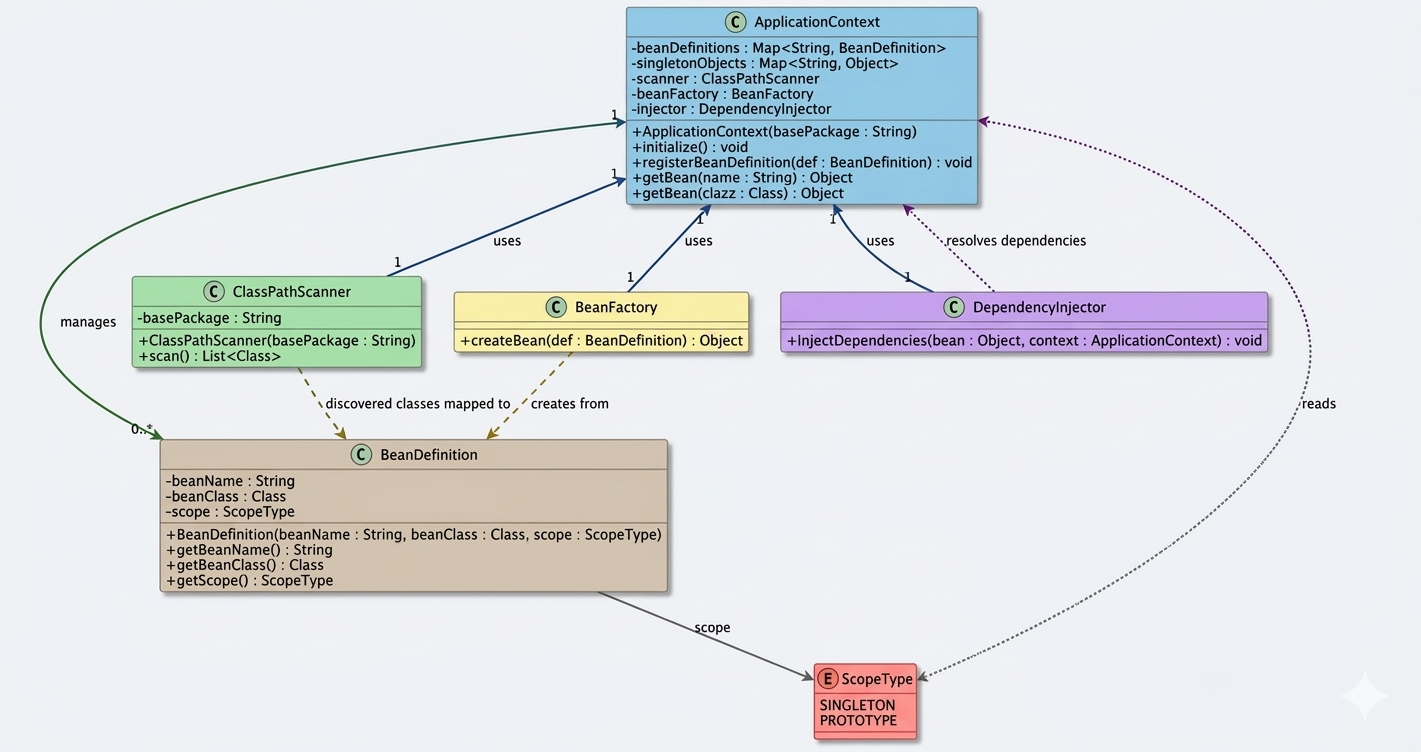
\includegraphics[width=0.8\textwidth]{images/class_gm.png}
    \caption{Annotation-д суурилсан DI framework-ийн классын диаграмм}
    \label{fig:class-diagram}
\end{figure}
~\ref{fig:class-diagram}-р зурагт annotation-д суурилсан
DI framework-ийн классын диаграммыг харуулав. Диаграммд
\texttt{ApplicationContext}, \texttt{ClassPathScanner},
\texttt{BeanFactory}, \texttt{BeanDefinition},
\texttt{DependencyInjector}, \texttt{ScopeType} гэсэн
зургаан үндсэн бүрэлдэхүүн хэсэг болон тэдгээрийн
харилцан хамаарал тусгагдсан байна.

\texttt{ApplicationContext} нь framework-ийн төв класс
бөгөөд \texttt{beanDefinitions}, \texttt{singletonObjects},
\texttt{scanner}, \texttt{beanFactory},
\texttt{injector} гэсэн таван хувийн талбар агуулна.
Энэ класс нь \texttt{ClassPathScanner},
\texttt{BeanFactory}, \texttt{DependencyInjector}
гурвыг \textit{uses} харилцаагаар ашиглах бөгөөд
\texttt{ClassPathScanner}-тэй \textit{manages}
харилцаагаар холбогдоно.

\texttt{ClassPathScanner} нь \texttt{basePackage}
талбартай бөгөөд \texttt{scan()} аргаар илэрсэн
классуудыг \texttt{BeanDefinition}-д харгалзуулан
\textit{discovered classes mapped to} харилцаагаар
дамжуулна. \texttt{BeanFactory} нь
\texttt{createBean()} аргаар \texttt{BeanDefinition}-д
тулгуурлан bean объект үүсгэх \textit{creates from}
үүрэгтэй.

\texttt{BeanDefinition} нь bean-ийн мета мэдээллийг
хадгалах \texttt{beanName}, \texttt{beanClass},
\texttt{scope} талбаруудтай бөгөөд \texttt{scope}
талбар нь \texttt{ScopeType} enum-тэй
\textit{scope} харилцаагаар холбогдоно.
\texttt{ScopeType} нь \texttt{SINGLETON} болон
\texttt{PROTOTYPE} гэсэн хоёр утгыг агуулна.
\texttt{DependencyInjector} нь
\texttt{ApplicationContext}-оос \textit{resolves
dependencies} болон \textit{reads} харилцаагаар
шаардлагатай bean-уудыг хайж inject хийнэ.
\section{Динамик загвар}
\subsection{Framework хэрэглэгчийн ажлын явцын загвар (Use case)}

Framework-ийн үндсэн actor нь хөгжүүлэгч байна.

\begin{itemize}
    \item Систем -- Annotation-д суурилсан DI Framework
    \item Actor -- Хөгжүүлэгч
\end{itemize}

Хөгжүүлэгчийн framework-тэй харилцах үндсэн ажлын явцууд:

\begin{itemize}
    \item Container эхлүүлэх
    \item Component class-уудыг scan хийх
    \item Bean бүртгэх
    \item Dependency injection хийх
    \item Bean-ийг container-оос авах
\end{itemize}
\begin{figure}[H]
    \centering
    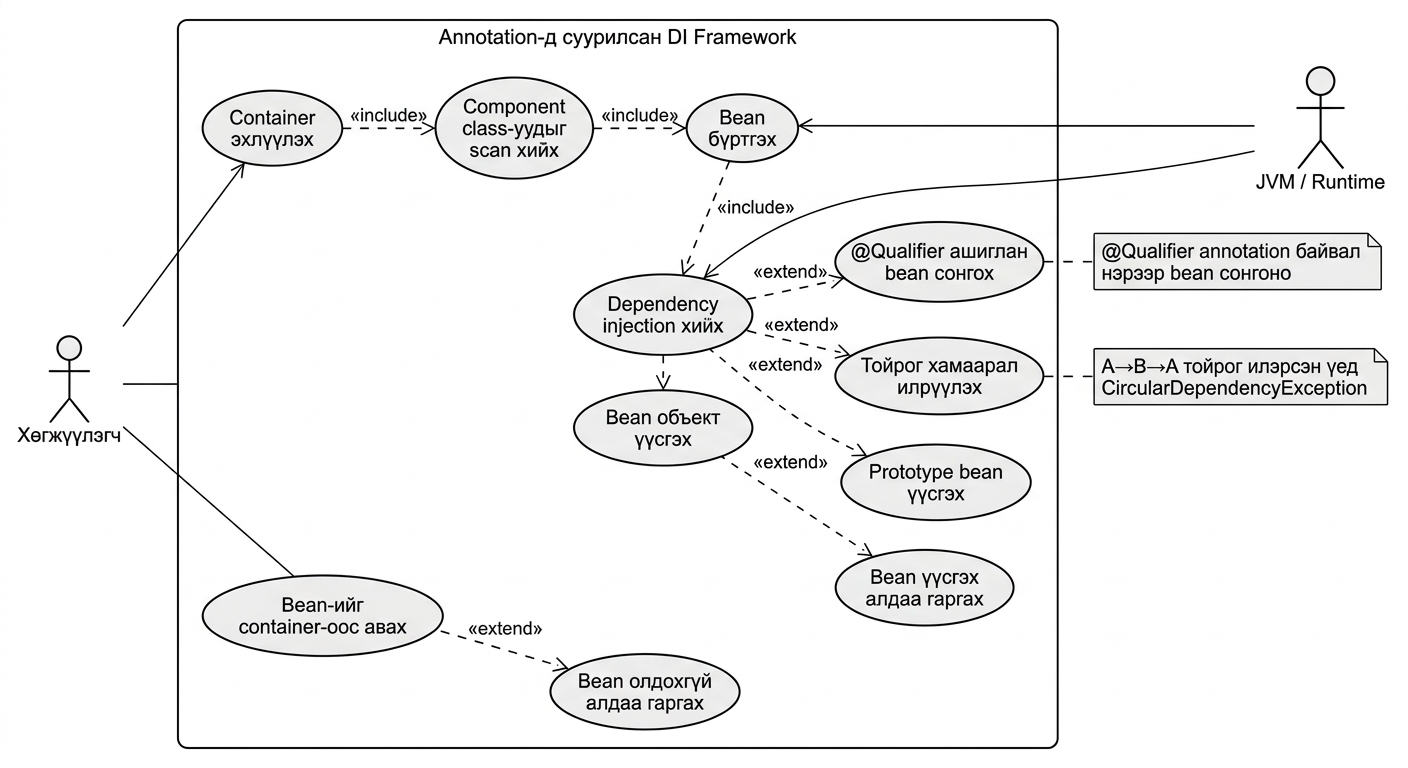
\includegraphics[width=0.6\textwidth]{images/use_case1.png}
    \caption{Use case}
    \label{fig:use_case1}
\end{figure}

~\ref{fig:use_case1}-р зурагт хөгжүүлэгч болон JVM actor - уудын ажлын явцын диаграммыг харуулсан.
\subsection{Ажлын явцын задаргаа (Use case description)}

\subsubsection{Container эхлүүлэх}

\begin{table}[H]
\centering
\caption{Container эхлүүлэх use case-ийн тодорхойлолт}
\label{tab:usecase-container-init}
\renewcommand{\arraystretch}{1.3}
\begin{tabular}{|p{3cm}|p{11cm}|}
\hline
Ажлын явц & Container эхлүүлэх \\ \hline
Тайлбар & Хөгжүүлэгч framework-ийн \texttt{ApplicationContext} объектыг үүсгэж container-ийг эхлүүлнэ. \\ \hline
Actor & Хөгжүүлэгч \\ \hline
Урьдчилсан нөхцөл & Package нэр болон framework-ийн үндсэн тохиргоо өгөгдсөн байна. \\ \hline
Үндсэн алхам & 
1. Хөгжүүлэгч \texttt{ApplicationContext} үүсгэнэ. \newline
2. Framework package scanning хийнэ. \newline
3. \texttt{@Component} annotation-тай классуудыг илрүүлнэ. \newline
4. BeanDefinition үүсгэж container-д бүртгэнэ. \newline
5. Шаардлагатай singleton bean-үүдийг үүсгэнэ. \\ \hline
Үр дүн & Framework ашиглахад бэлэн container үүссэн байна. \\ \hline
\end{tabular}
\end{table}

\subsubsection{Bean авах}

\begin{table}[H]
\centering
\caption{Bean авах use case-ийн тодорхойлолт}
\label{tab:usecase-getbean}
\renewcommand{\arraystretch}{1.3}
\begin{tabular}{|p{3cm}|p{11cm}|}
\hline
Ажлын явц & Bean авах \\ \hline
Тайлбар & Хөгжүүлэгч container-оос шаардлагатай bean-ийг нэрээр эсвэл төрлөөр авна. \\ \hline
Actor & Хөгжүүлэгч \\ \hline
Урьдчилсан нөхцөл & Container амжилттай эхэлсэн, bean бүртгэгдсэн байна. \\ \hline
Үндсэн алхам &
1. Хөгжүүлэгч \texttt{getBean()} аргыг дуудна. \newline
2. Framework bean definition-ийг шалгана. \newline
3. Singleton бол хадгалсан instance буцаана. \newline
4. Prototype бол шинэ instance үүсгэнэ. \\ \hline
Үр дүн & Хүссэн bean хөгжүүлэгчид буцаагдана. \\ \hline
\end{tabular}
\end{table}

\subsection{Бүлгийн дүгнэлт}

Энэхүү бүлэгт framework-ийн шаардлагыг тодорхойлов. Үүнд framework-ийн функциональ болон функциональ бус шаардлагууд, хөгжүүлэгчийн ашиглах үндсэн use case-ууд, мөн framework-ийг бүрдүүлэх үндсэн классууд, КҮХ карт, классын диаграммын бүтэц зэргийг системтэйгээр тодорхойлсон. Эдгээр нь дараагийн бүлэгт хэрэгжүүлэлт болон туршилтын хэсгийг боловсруулах суурь болно.